\documentclass{article}

\usepackage[main,final]{neurips_2026}

\usepackage[utf8]{inputenc}
\usepackage[T1]{fontenc}
\usepackage{hyperref}
\usepackage{url}
\usepackage{booktabs}
\usepackage{amsfonts}
\usepackage{amsmath,amssymb}
\usepackage{graphicx}
\usepackage{xcolor}
\usepackage{enumitem}
\usepackage{array}
\usepackage{multirow}
\usepackage{microtype}

\graphicspath{{figures/}}
\setlist[itemize]{leftmargin=1.3em, topsep=2pt, itemsep=1pt, parsep=0pt}
\setlist[enumerate]{leftmargin=1.5em, topsep=2pt, itemsep=1pt, parsep=0pt}

\title{PRISM: Probing Retrieval Inadequacy via Structural Mismatch}

\author{%
Ritik \quad Omkar \quad Vaishnavi \quad Moin \\
Arizona State University \\
CSE 579: Knowledge Representation and Reasoning \\
\url{https://github.com/ritwiz06/PRISM-Probing-Retrieval-Inadequacy-via-Structural-Mismatch}
}

\begin{document}

\maketitle

\begin{abstract}
PRISM is a representation-aware question answering system for studying retrieval failures caused by structural mismatch. Instead of sending every query to one retriever, PRISM routes each query to BM25, Dense, KG, or Hybrid retrieval using a production heuristic called computed Representation Adequacy Score (computed\_ras). The system exposes evidence provenance and reasoning traces, then evaluates routing and answer quality across curated, held-out, public-source, adversarial, human-evaluation, and open-corpus settings. The main empirical finding is that representation-aware routing is reliable on stable benchmark layers, while hard adversarial cases show that route adequacy alone is insufficient; calibrated evidence rescue remains the strongest research overlay on hard-case answer accuracy. Production routing therefore remains computed\_ras, while RAS\_V3, RAS\_V4, and calibrated rescue are reported as analysis or demo layers.
\end{abstract}

\section{Introduction and Motivation}

Many retrieval-augmented QA systems treat retrieval as a single ranking problem. PRISM starts from a different observation: some failures occur because the query was matched to the wrong \emph{representation}. An exact identifier query may need lexical matching, a paraphrased concept may need dense retrieval, a class-membership question may need a graph, and a bridge question may need fused text and structure. PRISM asks whether a system can detect this structural mismatch before retrieval and route the query accordingly.

The central contribution is an explicit, inspectable routing framework for representation-aware retrieval. PRISM is not a general web search engine. It is a bounded corpus, source-pack, and runtime-corpus QA workspace built to make route choice, evidence provenance, and reasoning traces visible.

\section{Background and Related Work}

PRISM combines ideas from sparse retrieval, dense retrieval, knowledge graphs, and retrieval-augmented generation. BM25 remains a strong lexical baseline for exact terms and identifiers \cite{robertson2009probabilistic}. Dense sentence embeddings such as Sentence-BERT support semantic similarity and paraphrase matching \cite{reimers2019sentence}. Knowledge graphs and RDF-style representations provide explicit entities, relations, and provenance for deductive reasoning \cite{hogan2021knowledge}. Modern RAG systems combine retrieval and generation, but often leave representation choice implicit \cite{lewis2020retrieval}. PRISM treats representation choice as a first-class KRR decision.

\section{Problem Formulation}

Let $x$ be a query and let $\mathcal{R}=\{\text{bm25}, \text{dense}, \text{kg}, \text{hybrid}\}$ be the route family set. PRISM selects a route
\[
    r^*(x) = \arg\max_{r \in \mathcal{R}} s_r(x),
\]
retrieves evidence $E_{r^*}(x)$, and produces an answer grounded in that evidence. The route should match the query's structural requirement:
\begin{itemize}
    \item lexical / identifier-heavy queries should route to BM25;
    \item semantic / paraphrastic queries should route to Dense retrieval;
    \item deductive / class-property queries should route to KG retrieval;
    \item relational / multi-hop queries should route to Hybrid retrieval.
\end{itemize}

The evaluation measures route accuracy, answer accuracy, evidence hit@k, top-1 evidence hit where available, and human judgments of evidence and trace quality.

\section{KRR Framing}

The KRR framing is structural mismatch. A query can be answerable in the corpus while still failing if the system chooses an inadequate representation. PRISM formalizes this with \emph{representation adequacy}: a route is adequate when its representation can preserve the relations, identifiers, abstractions, or multi-hop structure required by the query.

This framing makes the reasoning process explicit. PRISM does not only retrieve text; it reasons about the form of the query, selects the representation that should preserve the needed structure, retrieves evidence with provenance, and exposes a trace that links the final answer back to evidence ids.

\section{PRISM System Design}

\begin{figure}[t]
    \centering
    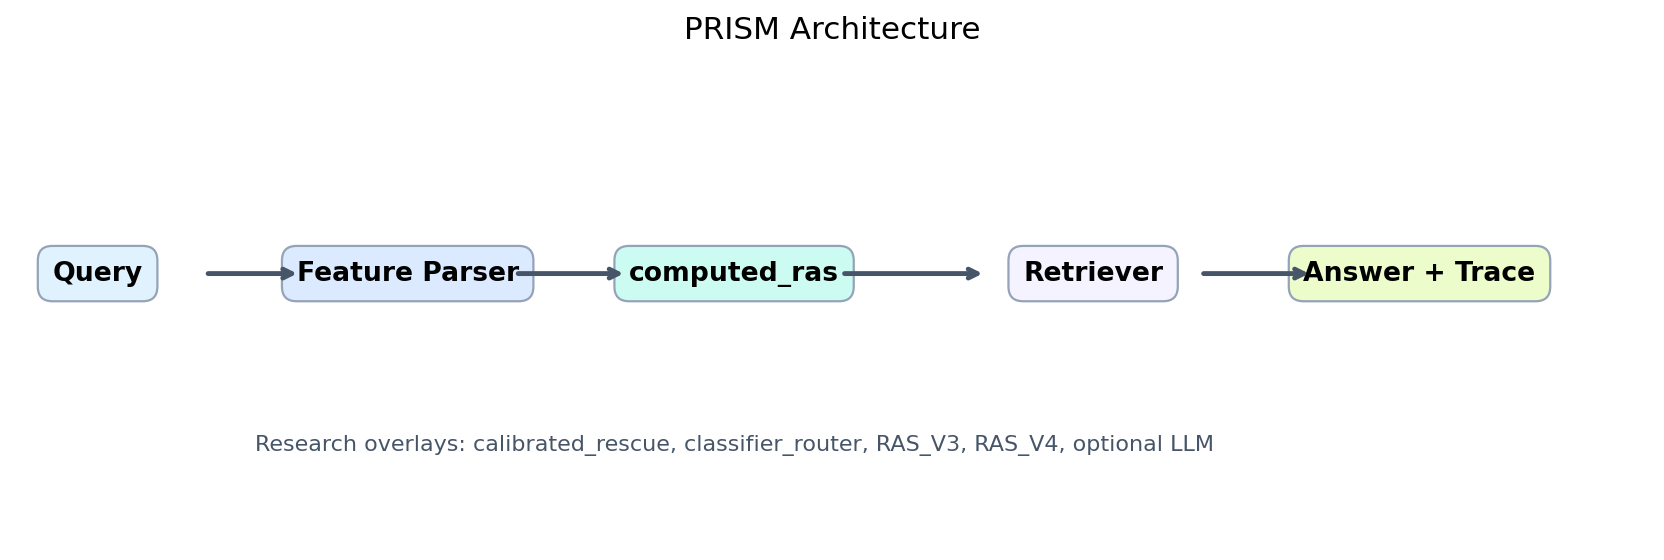
\includegraphics[width=0.95\linewidth]{architecture_diagram.png}
    \caption{PRISM architecture. Query features feed the production router, which selects BM25, Dense, KG, or Hybrid retrieval. Evidence, provenance, and traces are surfaced in the demo and evaluation artifacts.}
    \label{fig:architecture}
\end{figure}

The production pipeline has six stages: query feature extraction, route scoring, backend selection, evidence retrieval, answer synthesis, and trace generation. The Streamlit workspace exposes the same flow through demo, open-corpus, route-comparison, RAS-explainer, human-eval, and results views.

\section{Representation Adequacy Score}

PRISM's routing family is summarized in Table~\ref{tab:rasversions}. The production router is computed\_ras. It is a deterministic heuristic that assigns route penalties from query features and selects the minimum-penalty route. This makes the default path reproducible and interpretable.

RAS\_V3 and RAS\_V4 are research models. RAS\_V3 formalizes route adequacy as an interpretable feature-based model. RAS\_V4 extends the idea to joint route-and-evidence adequacy, because adversarial results show that route choice alone does not fully determine answer quality. Calibrated rescue is not a RAS replacement; it is an overlay that improves hard-case answerability by using calibration and top-k evidence rescue.

\begin{table}[t]
\centering
\small
\begin{tabular}{p{0.17\linewidth}p{0.22\linewidth}p{0.28\linewidth}p{0.18\linewidth}}
\toprule
\textbf{Variant} & \textbf{Model type} & \textbf{Main signal} & \textbf{Release status} \\
\midrule
computed\_ras & Deterministic heuristic & Query-feature penalties for BM25, Dense, KG, and Hybrid route families & Production default \\
computed\_ras\_v2 & Heuristic refinement & Narrow hard-case signals and ambiguity heuristics & Analysis-only \\
ras\_v3 & Interpretable linear route model & Feature contributions for route adequacy & Analysis-only \\
ras\_v4 & Interpretable joint adequacy model & Route adequacy plus evidence adequacy diagnostics & Analysis-only \\
calibrated\_rescue & Overlay, not a RAS replacement & Dev-tuned route calibration and top-k evidence rescue & Research/demo overlay \\
\bottomrule
\end{tabular}
\caption{RAS family comparison. The production decision remains explicit: \texttt{computed\_ras} is the default router; later variants are reported as analysis layers.}
\label{tab:rasversions}
\end{table}

\begin{table}[t]
\centering
\small
\begin{tabular}{p{0.24\linewidth}p{0.20\linewidth}p{0.43\linewidth}}
\toprule
\textbf{Component} & \textbf{Role} & \textbf{Interpretation} \\
\midrule
computed\_ras & Production router & Stable deterministic router used by default across the demo and benchmark-safe path. \\
calibrated\_rescue & Research/demo overlay & Improves adversarial answer accuracy by using calibration and top-k evidence rescue. \\
classifier\_router & Baseline & Learned comparison router for measuring route-boundary behavior. \\
ras\_v3 & Analysis-only model & Formalizes route adequacy with interpretable feature contributions. \\
ras\_v4 & Analysis-only model & Adds evidence adequacy to explain why route choice alone is insufficient on hard cases. \\
optional LLM & Experimental layer & Local-only optional comparison path; not part of the core production runtime. \\
\bottomrule
\end{tabular}
\caption{Production versus research distinction used throughout PRISM.}
\label{tab:prodresearch}
\end{table}


\section{Retrieval Backends}

PRISM uses four backend families:
\begin{itemize}
    \item \textbf{BM25}: lexical retrieval for exact identifiers, formal names, and code-like strings.
    \item \textbf{Dense}: sentence-transformer and FAISS-backed retrieval for semantic and paraphrastic queries.
    \item \textbf{KG}: RDF/graph-style evidence for class, property, and membership reasoning.
    \item \textbf{Hybrid}: fused retrieval for bridge and multi-hop cases that need both text and structure.
\end{itemize}

\section{Reasoning Trace and Evidence Provenance}

Every answer is paired with evidence ids and a route rationale. This is important for KRR because the system's answer should be inspectable: the route explains why a representation was selected, and the evidence trace explains what supports the answer. Universal or scope-heavy claims require the trace to show support or counterexample handling where available.

\section{Evaluation Setup}

PRISM is evaluated through multiple layers:
\begin{itemize}
    \item curated 80-example end-to-end benchmark;
    \item 32-example external mini-benchmark;
    \item generalization\_v2 with clean and noisy variants;
    \item extracted-KG and structure-shift evaluation;
    \item public raw-document corpus and public graph grounding;
    \item adversarial hard-case benchmark;
    \item standard and comparative human evaluation;
    \item open-corpus smoke evaluation.
\end{itemize}

The release artifacts under \texttt{data/eval/}, \texttt{data/human\_eval/}, and \texttt{data/final\_release/} are the source of truth for all numbers in this report.

\section{Results}

\begin{table}[t]
\centering
\small
\begin{tabular}{lccc}
\toprule
\textbf{Evaluation layer} & \textbf{Size / split} & \textbf{Route acc.} & \textbf{Answer acc.} \\
\midrule
Curated end-to-end & 80 examples & 1.000 & 1.000 \\
External mini-benchmark & 32 examples & 1.000 & 1.000 \\
Generalization v2 clean test & 40 test examples & 0.950 & 1.000 \\
Generalization v2 noisy test & 40 test examples & 0.950 & 0.975 \\
Public raw-document test & 24 test examples & 0.917 & 1.000 \\
Public graph test & 16 test examples & 1.000 & 1.000 \\
Adversarial test & 24 test examples & 0.750 & 0.917 \\
Open-corpus smoke & 5 smoke queries & -- & 1.000 \\
\bottomrule
\end{tabular}
\caption{Release-level PRISM benchmark summary. Values are copied from the existing evaluation artifacts under \texttt{data/eval/} and \texttt{data/final\_release/}.}
\label{tab:benchmarks}
\end{table}


\begin{figure}[t]
    \centering
    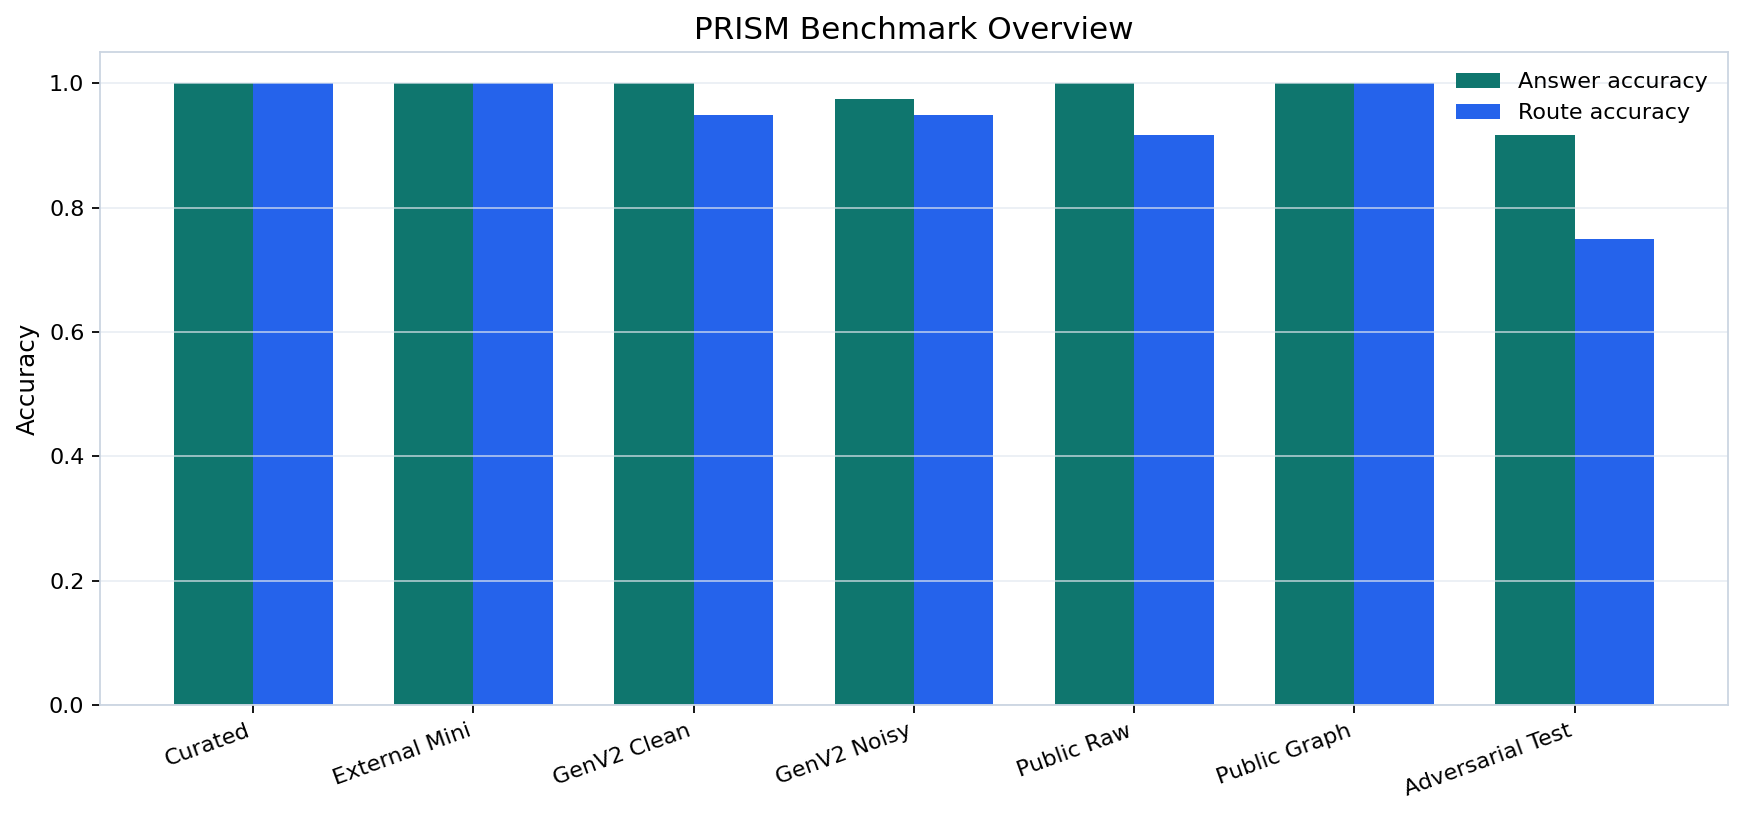
\includegraphics[width=0.95\linewidth]{benchmark_overview.png}
    \caption{Benchmark overview generated from final release artifacts. Stable benchmark layers are strong, while hard adversarial cases remain the most informative weakness.}
    \label{fig:benchmarks}
\end{figure}

Table~\ref{tab:benchmarks} shows that computed\_ras is stable on curated, external, held-out, public raw, public graph, and open-corpus smoke checks. The adversarial benchmark is intentionally harder and exposes route-boundary errors, misleading lexical cues, and evidence ranking failures.

\begin{table}[t]
\centering
\small
\begin{tabular}{lccc}
\toprule
\textbf{System} & \textbf{Status} & \textbf{Route acc.} & \textbf{Answer acc.} \\
\midrule
computed\_ras & Production & 0.750 & 0.917 \\
calibrated\_rescue & Research overlay & 0.875 & 0.958 \\
classifier\_router & Research baseline & 0.792 & 0.875 \\
ras\_v3 & Analysis-only & 0.833 & 0.917 \\
ras\_v4 & Analysis-only & 0.750 & 0.917 \\
ras\_v4 + rescue & Research overlay & 0.750 & 0.958 \\
\bottomrule
\end{tabular}
\caption{Adversarial test comparison. Calibrated rescue is strongest on hard-case answer accuracy, but it is retained as a research/demo overlay rather than replacing the production router.}
\label{tab:adversarial}
\end{table}


\begin{figure}[t]
    \centering
    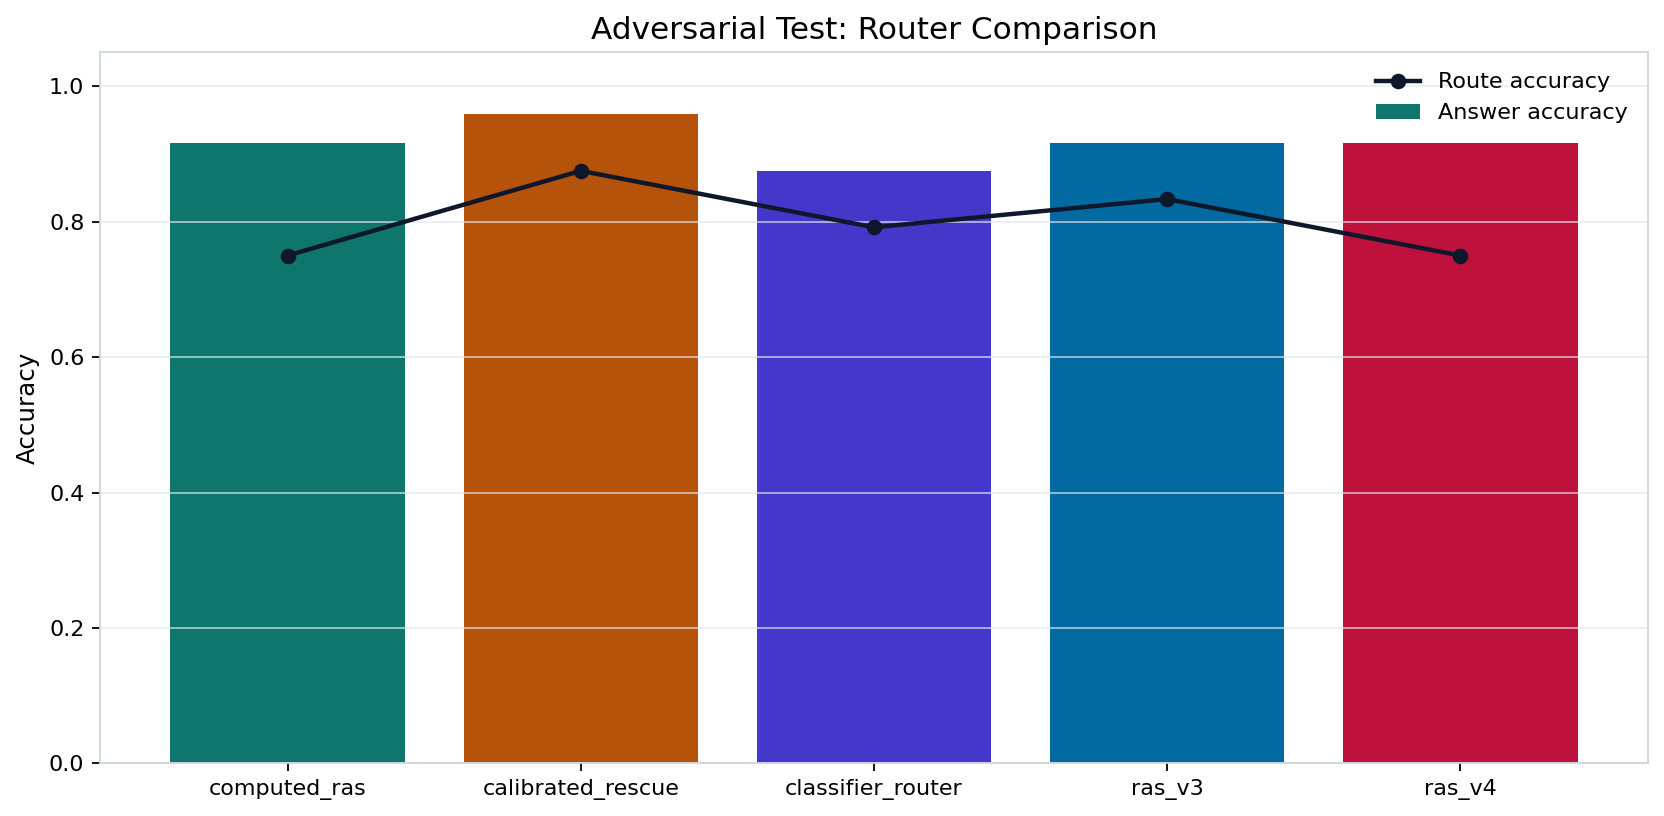
\includegraphics[width=0.95\linewidth]{adversarial_router_comparison.png}
    \caption{Adversarial router comparison. Calibrated rescue is strongest on hard-case answer accuracy, while computed\_ras remains the production default under the release guardrails.}
    \label{fig:adversarial}
\end{figure}

\section{Human Evaluation}

The standard human-eval packet contains 36 items annotated by 4 evaluators. The comparative packet contains 28 pairwise items with 112 annotations. Table~\ref{tab:human} summarizes the standard rubric means.

\begin{table}[t]
\centering
\small
\begin{tabular}{lc}
\toprule
\textbf{Human-eval dimension} & \textbf{Mean score} \\
\midrule
Route appropriateness & 2.896 \\
Evidence sufficiency & 2.917 \\
Answer faithfulness & 2.917 \\
Trace faithfulness & 2.931 \\
Trace clarity & 2.944 \\
Overall usefulness & 2.875 \\
\bottomrule
\end{tabular}
\caption{Standard human-evaluation results from 4 annotators over a 36-item packet. Scores use the existing ordinal rubric artifacts in \texttt{data/human\_eval/}.}
\label{tab:human}
\end{table}


Human judgments generally support evidence and trace usefulness, but the packet is small and subjective. Comparative evaluation shows many ties between computed\_ras and research overlays, while calibrated rescue is preferred on a small subset of hard comparisons. These results support the project narrative without justifying a production-router change.

\begin{figure}[t]
    \centering
    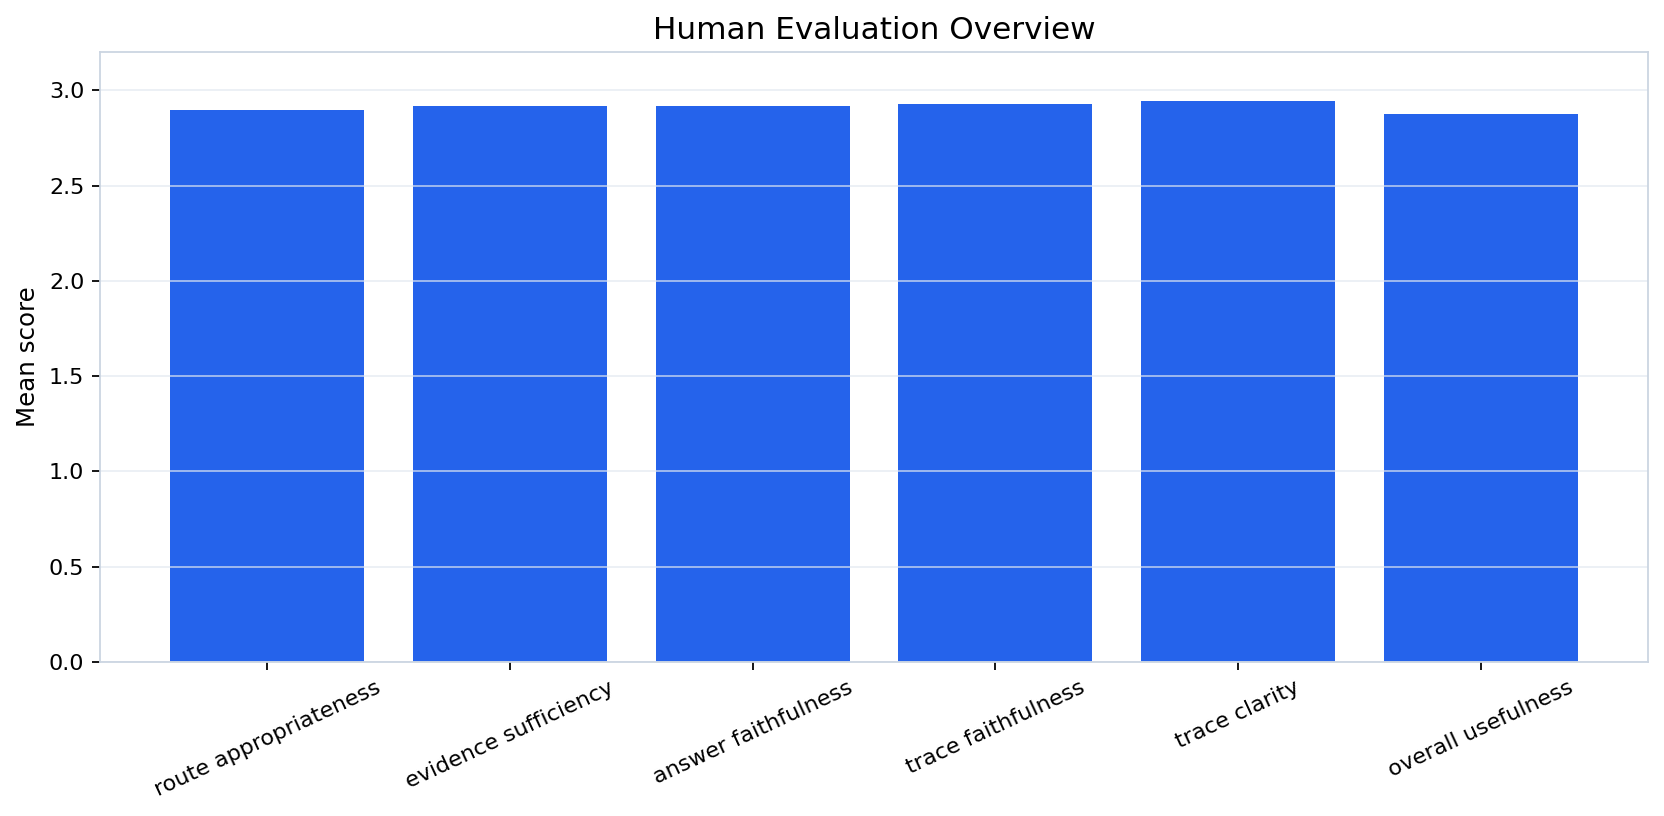
\includegraphics[width=0.9\linewidth]{human_eval_overview.png}
    \caption{Human-eval score overview. Scores are high on trace clarity and faithfulness, with threats to validity from small sample size and evaluator subjectivity.}
    \label{fig:human}
\end{figure}

\section{UI, Demo, and Open-Corpus Workspace}

The Streamlit app exposes the final system through an executive summary, guided demo, RAS explainer, query view, open-corpus workspace, router comparison page, evidence/graph view, human-eval view, and results/paper view. The open-corpus layer supports bounded source packs, local folders, URL lists, and runtime corpora while keeping these artifacts separate from benchmark corpora.

\section{Limitations}

PRISM has four important limitations. First, it is not arbitrary web-scale search. Second, adversarial route-boundary cases remain difficult. Third, calibrated rescue improves hard-case answer accuracy by using post-route evidence, showing that route adequacy alone is not enough. Fourth, human evaluation is useful but limited by packet size, evaluator pool, and ordinal-subjective judgments.

\section{Conclusion and Future Work}

PRISM demonstrates that representation-aware retrieval routing is a useful KRR framing for retrieval-augmented QA. The system is stable on benchmark-safe settings, exposes evidence and route reasoning, and honestly identifies adversarial hard cases as the remaining weakness. Future work should focus on stronger uncertainty-aware routing, better evidence adequacy modeling, larger human studies, and more robust open-corpus source-pack evaluation.

\section*{Contribution Table}

\begin{table}[h]
    \centering
    \small
    \begin{tabular}{p{0.16\linewidth} p{0.60\linewidth} p{0.15\linewidth}}
        \toprule
        \textbf{Member} & \textbf{Contribution} & \textbf{Role} \\
        \midrule
        Ritik & Production integration; routing and demo stability; final report; release package; presentation deliverables; benchmark-safe acceptance. & Lead / integration \\
        Omkar & TBD by teammate. & TBD \\
        Vaishnavi & TBD by teammate. & TBD \\
        Moin & TBD by teammate. & TBD \\
        \bottomrule
    \end{tabular}
    \caption{Project contribution summary.}
\end{table}

\bibliographystyle{plain}
\bibliography{references}

\end{document}
